\documentclass{ximera}

\newcommand{\RR}{\mathbb R}
\renewcommand{\d}{\,d}
\newcommand{\dd}[2][]{\frac{d #1}{d #2}}
\renewcommand{\l}{\ell}
\newcommand{\ddx}{\frac{d}{dx}}
\newcommand{\dfn}{\textbf}
\newcommand{\eval}[1]{\bigg[ #1 \bigg]}


\outcome{Define a cross product.}
\outcome{Compute cross products.}
\outcome{Use cross products in applied settings.}

\title[Dig-In:]{The cross product}

\begin{document}
\begin{abstract}
  The cross product is a special way to multiply two vectors in
  three-dimensional space.
\end{abstract}
\maketitle

There is no ``nice'' way to ``multiply'' two vectors and obtain
another vector in general. However, in the special case of $\R^3$,
there is an important multiplication operation called ``the cross
product.''

The cross product is linked inextricably to the determinant, so we
will first introduce the determinant before introducing this new
operation. See \link[this paper]{http://www-groups.dcs.st-and.ac.uk/history/HistTopics/Matrices_and_determinants.html}
for a discussion of the history of the idea of a \textit{determinant}.

\section{Determinants}

\begin{definition}
  Given a $2\times2$ matrix, the \dfn{determinant} is given by:
  \[
  \det
  \begin{bmatrix}
    a & b\\
    c & d
  \end{bmatrix}
  =
  \begin{vmatrix}
    a & b\\
    c & d
  \end{vmatrix}
  = ad -bc.
  \]
\end{definition}
Why would anyone ever be interested in this? Well to start, given nonzero vectors
\[
\vec{v} = \vector{a,b}\quad\text{and}\quad\vec{w}=\vector{c,d}
\]
we can form a parallelogram:
\begin{image}
\begin{tikzpicture}
  \draw[fill=fill1!50!white,draw=none]
  (0, 0)         % starting point
  -- ++(5,1)     % move along this vector
  -- ++(2,3)     % then along this vector
  -- ++(-5,-1)   % then back along that vector
  -- cycle;      % and back to where you started
  \draw[->,ultra thick,penColor] (0,0) -- (5,1);
  \draw[->,ultra thick,penColor2] (0,0) -- (2,3);
  \draw[->,ultra thick,dashed,penColor2] (5,1) -- (7,4);
  \draw[->,ultra thick,dashed,penColor] (2,3) -- (7,4);
  \node[above,penColor] at (2.5,.5) {$\vec{v}$}; %% <a,b>
  \node[below right,penColor2] at (1,1.5) {$\vec{w}$}; %% <c,d>
\end{tikzpicture}
\end{image}
The determinant gives the (signed) area of this parallelogram, where
the sign of the area is given by the sign of the angle between
$\vec{v}$ and $\vec{w}$. To understand why this is true, make a
rectangle around the parallelogram:
\begin{image}
\begin{tikzpicture}
  \draw[fill=fill1!50!white,draw=none]
  (0, 0)         % starting point
  -- ++(5,1)     % move along this vector
  -- ++(2,3)     % then along this vector
  -- ++(-5,-1)   % then back along that vector
  -- cycle;      % and back to where you started

  \draw[fill=fill5] (5, 0) -- (7,0) -- (7,1) -- (5,1) -- cycle;
  \draw[fill=fill5] (0, 3) -- (2,3) -- (2,4) -- (0,4) -- cycle;

  \draw[fill=fill3] (0, 0) -- (5,0) -- (5,1) -- cycle;
  \draw[fill=fill3] (2,3) -- (7,4) -- (2,4) -- cycle;

  \draw[fill=fill4] (0, 0) -- (2,3) -- (0,3) -- cycle;
  \draw[fill=fill4] (5, 1) -- (7,1) -- (7,4) -- cycle;
  
  \draw[->,ultra thick,penColor] (0,0) -- (5,1);
  \draw[->,ultra thick,penColor2] (0,0) -- (2,3);
  \draw[->,ultra thick,dashed,penColor2] (5,1) -- (7,4);
  \draw[->,ultra thick,dashed,penColor] (2,3) -- (7,4);

  \draw[decoration={brace,mirror,raise=.1cm},decorate,thin] (0,0)--(5,0);
  \node[below] at (2.5,-.2) {$a$};

  \draw[decoration={brace,mirror,raise=.1cm},decorate,thin] (7,4)--(2,4);
  \node[above] at (4.5,4.2) {$a$};

  \draw[decoration={brace,mirror,raise=.1cm},decorate,thin] (7,0)--(7,1);
  \node[right] at (7.2,.5) {$b$};

  \draw[decoration={brace,mirror,raise=.1cm},decorate,thin] (0,4)--(0,3);
  \node[left] at (-.2,3.5) {$b$};

  \draw[decoration={brace,mirror,raise=.1cm},decorate,thin] (7,1)--(7,4);
  \node[right] at (7.2,2.5) {$d$};

  \draw[decoration={brace,mirror,raise=.1cm},decorate,thin] (0,3)--(0,0);
  \node[left] at (-.2,1.5) {$d$};

  \draw[decoration={brace,mirror,raise=.1cm},decorate,thin] (0,3)--(0,0);
  \node[left] at (-.2,1.5) {$d$};

  \draw[decoration={brace,raise=.1cm},decorate,thin] (0,4)--(2,4);
  \node[above] at (1,4.2) {$c$};

  \draw[decoration={brace,mirror,raise=.1cm},decorate,thin] (5,0)--(7,0);
  \node[below] at (6,-.2) {$c$};
  
  \node[above,penColor] at (2.5,.5) {$\vec{v}$}; %% <a,b>
  \node[below right,penColor2] at (1,1.5) {$\vec{w}$}; %% <c,d>
\end{tikzpicture}
\end{image}
Now we see that the area of the parallelogram is
\[
\text{Area of rectangle} - \text{Area of other regions}
\]
and this is
\begin{align*}
  (a+c)(b+d) - \left(cd + ab -2bc \right)&= ab + ad + bc + cd - cd - ab-2bc\\
  &=  ad - bc\\
  &= \det
  \begin{bmatrix}
    a & b\\
    c & d
  \end{bmatrix}.
\end{align*}

Typically when one computes the determinant of a $2\times 2$ matrix,
we think of the terms as follows:
\begin{image}[1in]
  \begin{tikzpicture}
    \matrix (mtrx)  [matrix of math nodes,ampersand replacement=\&,%column sep=.1em,
      nodes={text height=1ex,text width=2ex}]
            {
              a \& b \\
              c \& d \\
            };
            \draw[thick] (mtrx-1-1.north) -| (mtrx-2-1.south west)
            -- (mtrx-2-1.south);
            \draw[thick] (mtrx-1-2.north) -| (mtrx-2-2.south east)
            -- (mtrx-2-2.south);
            \draw[ultra thick,red!20!white,->]
            (mtrx-1-2.center) -- (mtrx-2-1.center);
            \draw[draw,ultra thick,blue!20!white,->]
            (mtrx-1-1.center)  --  (mtrx-2-2.center);
            \matrix (mtrx2)  [matrix of math nodes,ampersand replacement=\&,nodes={text height=1ex,text width=2ex}]
            {
              a \& b\\
              c \& d\\
            };
            \node at (0,-.7) {${\color{blue!50!black}ad}-{\color{red!50!black}bc}$};
  \end{tikzpicture}
\end{image}


\begin{definition}
  Given a $3\times 3$ matrix, the \dfn{determinant} is given by
  \begin{align*}
  &\det\begin{bmatrix}
  a_1 &  a_2 & a_3 \\
  b_1 &  b_2 & b_3 \\
  c_1 &  c_2 & c_3
  \end{bmatrix}
  =
  \begin{vmatrix}
    a_1 &  a_2 & a_3 \\
    b_1 &  b_2 & b_3 \\
    c_1 &  c_2 & c_3
  \end{vmatrix}\\
  &= a_1b_2c_3+b_1c_2a_3+c_1a_2b_3-a_3b_2c_1-b_3c_2a_1-c_3a_2b_1.
  \end{align*}
\end{definition}
We can remember this formula by writing the first two columns of the
matrix to the right of the matrix, and using either of the two
following patterns:
\begin{image}
\begin{tikzpicture}
\node at (0,0) {$\det
\begin{bmatrix}
  a_1 & a_2 & a_3\\
  b_1 & b_2 & b_3\\
  c_1 & c_2 & c_3
\end{bmatrix}
= a_1
\begin{vmatrix}
  b_2 & b_3\\
  c_2 & c_3
\end{vmatrix}
-a_2
\begin{vmatrix}
  b_1 & b_3\\
  c_1 & c_3
\end{vmatrix}
+a_3
\begin{vmatrix}
  b_1 & b_2\\
  c_1 & c_2
\end{vmatrix}$};

\draw[ultra thick,->,gray] (-.27,-1.3) -- (-.27,-.7);
\draw[ultra thick,->,gray] (1.76,-1.3) -- (1.76,-.7);
\draw[ultra thick,->,gray] (3.8,-1.3) -- (3.8,-.7);

\node at (-.27,-2) {\scalebox{.7}{
    $\begin{bmatrix}
      a_1 & \bullet & \bullet\\
      \bullet & b_2 & b_3\\
      \bullet & c_2 & c_3
    \end{bmatrix}$}};

\node at (1.76,-2) {\scalebox{.7}{
    $\begin{bmatrix}
      \bullet & a_2 & \bullet\\
      b_1 & \bullet & b_3\\
      c_1 & \bullet & c_3
    \end{bmatrix}$}};

\node at (3.8,-2) {\scalebox{.7}{
    $\begin{bmatrix}
      \bullet & \bullet & a_3\\
      b_1 & b_2 & \bullet\\
      c_1 & c_2 & \bullet
    \end{bmatrix}$}};
\end{tikzpicture}
\end{image}

Or:



%% Credit for the following image goes to
%% http://tex.stackexchange.com/a/257063
\begin{image}
  \begin{tikzpicture}
    \matrix (mtrx)  [matrix of math nodes,ampersand replacement=\&,column sep=1em, nodes={text height=1ex,text width=2ex}]
            {
              a_1 \& a_2 \& a_3 \& a_1 \& a_2         \\
              b_1 \& b_2 \& b_3 \& b_1 \& b_2         \\
              c_1 \& c_2 \& c_3 \& c_1 \& c_2         \\
            };
            \matrix (mtrx3)  [matrix of math nodes,ampersand replacement=\&,column sep=1em, nodes={text height=1ex,text width=2ex}] at (5,0)
            { 
              a_1 \& a_2 \& a_3 \& a_1 \& a_2         \\
              b_1 \& b_2 \& b_3 \& b_1 \& b_2         \\
              c_1 \& c_2 \& c_3 \& c_1 \& c_2         \\
            };
            \draw[thick] (mtrx-1-1.north) -| (mtrx-3-1.south west)
            -- (mtrx-3-1.south);
            \draw[thick] (mtrx-1-3.north) -| (mtrx-3-3.south east)
            -- (mtrx-3-3.south);
            \draw[ultra thick,red!20!white,->]
            (mtrx3-3-1.center) edge (mtrx3-1-3.center)
            (mtrx3-3-2.center) edge (mtrx3-1-4.center)
            (mtrx3-3-3.center)  --  (mtrx3-1-5.center);
            \draw[draw,ultra thick,blue!20!white,->]
            (mtrx-1-1.center) edge (mtrx-3-3.center)
            (mtrx-1-2.center) edge (mtrx-3-4.center)
            (mtrx-1-3.center)  --  (mtrx-3-5.center);
            \matrix (mtrx2)  [matrix of math nodes,ampersand replacement=\&,column sep=1em, nodes={text height=1ex,text width=2ex}]
            { 
              a_1 \& a_2 \& a_3 \& a_1 \& a_2         \\
              b_1 \& b_2 \& b_3 \& b_1 \& b_2         \\
              c_1 \& c_2 \& c_3 \& c_1 \& c_2         \\
            };
            \matrix (mtrx4)  [matrix of math nodes,ampersand replacement=\&,column sep=1em, nodes={text height=1ex,text width=2ex}] at (5,0)
            { 
              a_1 \& a_2 \& a_3 \& a_1 \& a_2         \\
              b_1 \& b_2 \& b_3 \& b_1 \& b_2         \\
              c_1 \& c_2 \& c_3 \& c_1 \& c_2         \\
            };
            \draw[thick] (mtrx4-1-1.north) -| (mtrx4-3-1.south west)
            -- (mtrx4-3-1.south);
            \draw[thick] (mtrx4-1-3.north) -| (mtrx4-3-3.south east)
            -- (mtrx4-3-3.south);
            \node at (2.5,-1) {${\color{blue!50!black}a_1b_2c_3}+{\color{blue!50!black}a_2b_3c_1}+{\color{blue!50!black}a_3b_1c_2}-{\color{red!50!black}a_3b_2c_1}-{\color{red!50!black}a_1b_3c_2}-{\color{red!50!black}a_2b_1c_3}$};
            \node at (0,1) {{\color{blue!50!black}positive terms}};
            \node at (5,1) {{\color{red!50!black}negative terms}};
  \end{tikzpicture}
\end{image}

\begin{question}
  Compute:
  \[
  \det
  \begin{bmatrix} 
    1 & 4 & 7\\
    2 & 5 & 8\\
    3 & 6 & 9\\
  \end{bmatrix}
  \begin{prompt}
    = \answer{0}
  \end{prompt}
  \]
\end{question}








\section{Cross products}

\begin{definition}
  The \dfn{cross product} of two vectors is given by: 
  \[
  \vector{a_1,a_2,a_3} \cross \vector{b_1,b_2,b_3} = \det
  \begin{bmatrix}
    \veci & \vecj & \veck\\
    a_1 & a_2 & a_3\\
    b_1 & b_2 & b_3
  \end{bmatrix}
  \]
\end{definition}
The first thing you should notice about the the cross product is that
\[
\mathbf{vector}\cross \mathbf{vector} = \mathbf{vector}.
\]
  When computing the cross product, the pattern:

  \begin{image}
\begin{tikzpicture}
\node at (0,0) {$\det
  \begin{bmatrix}
    \veci & \vecj & \veck\\
    a_1 & a_2 & a_3\\
    b_1 & b_2 & b_3
\end{bmatrix}
= \veci
\begin{vmatrix}
  a_2 & a_3\\
  b_2 & b_3
\end{vmatrix}
-\vecj
\begin{vmatrix}
  a_1 & a_3\\
  b_1 & b_3
\end{vmatrix}
+\veck
\begin{vmatrix}
  a_1 & a_2\\
  b_1 & b_2
\end{vmatrix}$};

\draw[ultra thick,->,gray] (-.27,-1.3) -- (-.27,-.7);
\draw[ultra thick,->,gray] (1.61,-1.3) -- (1.61,-.7);
\draw[ultra thick,->,gray] (3.58,-1.3) -- (3.58,-.7);

\node at (-.27,-2) {\scalebox{.7}{
    $\begin{bmatrix}
      \veci & \bullet & \bullet\\
      \bullet & a_2 & a_3\\
      \bullet & b_2 & b_3
    \end{bmatrix}$}};

\node at (1.61,-2) {\scalebox{.7}{
    $\begin{bmatrix}
      \bullet & \vecj & \bullet\\
      a_1 & \bullet & a_3\\
      b_1 & \bullet & b_3
    \end{bmatrix}$}};

\node at (3.58,-2) {\scalebox{.7}{
    $\begin{bmatrix}
      \bullet & \bullet & \veck\\
      a_1 & a_2 & \bullet\\
      b_1 & b_2 & \bullet
    \end{bmatrix}$}};
\end{tikzpicture}
  \end{image}
  
is usually most efficient, because you immediately have the
components of the desired vector, without additional
simplification.

\begin{question}
  Compute:
  \[
  \vector{2,3,1} \cross \vector{1,1,1}
  \begin{prompt}
    = \vector{\answer{2},\answer{-1},\answer{-1}}
  \end{prompt}
  \]
  \begin{question}
  Compute:
  \[
  \vector{1,1,1}\cross\vector{2,3,1} 
  \begin{prompt}
    = \vector{\answer{-2},\answer{1},\answer{1}}
  \end{prompt}
  \]
\end{question}
\end{question}

Note that the cross product is not commutative! In fact, it is
anticommutative:

\begin{theorem}[The Cross Product is Anticommutative]
  Given two vectors $\vec{a}$ and $\vec{b}$ in $\R^3$
  \[
  \vec{a} \cross\vec{b} = -\vec{b}\cross\vec{a}
  \]
\end{theorem}
The anticommutative property of the cross product demonstrates that
$\vec{a}\cross\vec{b}$ and $\vec{b}\cross\vec{a}$ differ only by a
sign. These vectors have the same magnitude but point in the opposite
direction. Now let's examine the cross product on famous unit vectors.
\begin{question}
  Compute:
  \[
  \veci \cross \vecj
  \begin{prompt}
    = \vector{\answer{0},\answer{0},\answer{1}}
  \end{prompt}
  \]
  \begin{question}
  Compute:
  \[
  \vecj\cross\veck 
  \begin{prompt}
    = \vector{\answer{1},\answer{0},\answer{0}}
  \end{prompt}
  \]
  \begin{question}
  Compute:
  \[
  \veck\cross\veci 
  \begin{prompt}
    = \vector{\answer{0},\answer{1},\answer{0}}
  \end{prompt}
  \]
\end{question}
\end{question}
\end{question}

One way to remember the relation between the cross product and the unit vectors $\veci$, $\vecj$, and $\veck$ is to use the diagram below:
\begin{image}[1in]
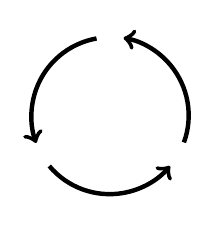
\begin{tikzpicture}
  \draw[ultra thick,->] (.94,-.34) arc (-20:80:1cm);
  \draw[ultra thick,->] (-.17,.98) arc (100:200:1cm);
  \draw[ultra thick,->] (-.77,-.64) arc (220:320:1cm);
  \node at (0,1) {$\veci$};
  \node at (-.87,-.5) {$\vecj$};
  \node at (.87,-.5) {$\veck$};
\end{tikzpicture}
\end{image}

Since we see that the cross product of two basic unit vectors produces
a vector orthogonal to \textit{both} unit vectors, we are lead to our
next theorem (which could be verified through brute force
computations).

\begin{theorem}
  The vector $\vec{a}\cross\vec{b}$ is orthogonal to both $\vec{a}$
  and $\vec{b}$.
\end{theorem}

When seeking a vector perpendicular to both $\vec a$ and $\vec b$, we
essentially have two directions to choose from, one in the direction
of $\vec{a}\cross\vec{b}$ and one in the direction of
$\vec{b}\cross\vec{a}$.  The direction of the cross product is given
by the \textit{right-hand rule}.  Given $\vec{a}$ and $\vec{b}$ in
$\R^3$ with the same initial point, point the index finger of your
right-hand in the direction of $\vec{a}$ and let your middle finger
point in the direction of $\vec{b}$ (much as we did when establishing
the right-hand rule for the 3-dimensional coordinate system). Your
thumb will naturally extend in the direction of
$\vec{a}\cross\vec{b}$.  If you switch, and point the index finder in
the direction of $\vec{b}$ and the middle finger in the direction of
$\vec{a}$, your thumb will now point in the opposite direction,
allowing you to ``visualize'' the anticommutative property of the
cross product.\index{right-hand rule}
\begin{image}[2in]
  %% Based on: https://commons.wikimedia.org/wiki/File:Right_hand_rule_cross_product.svg
  %% Which was based on: https://commons.wikimedia.org/wiki/File:Right_hand_cross_product.png
  %% Which was based on: https://commons.wikimedia.org/wiki/File:LeftHandOutline.png
  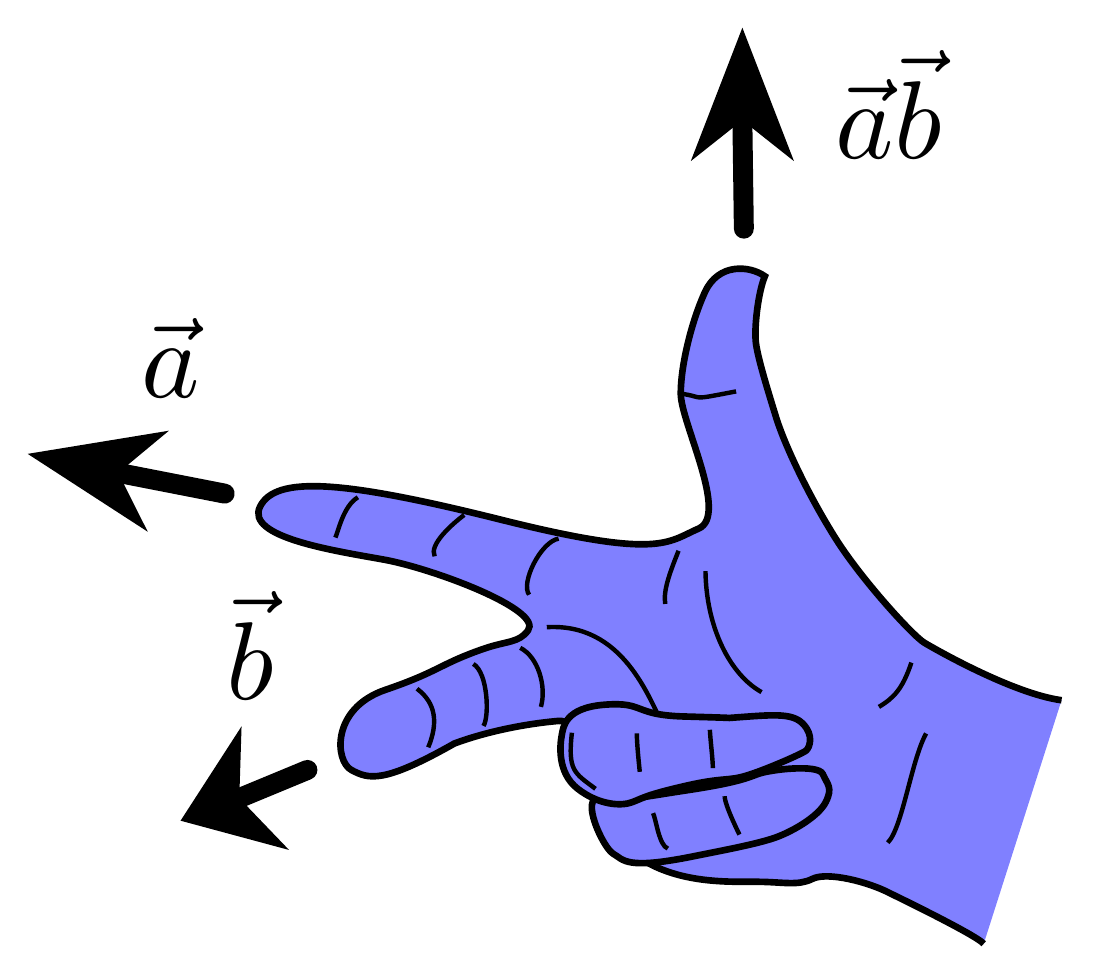
\begin{tikzpicture}[y=0.80pt, x=0.80pt, yscale=-1.000000, xscale=1.000000, inner sep=0pt, outer sep=0pt]
    \path[draw=black,fill=blue!50!white,line width=2.400pt] (466.9820,303.7880) ..
    controls (444.9820,300.7880) and (409.9820,280.7880) .. (404.9820,277.7880) ..
  controls (399.9820,274.7880) and (376.9820,249.7880) .. (364.9820,230.7880) ..
  controls (352.9820,211.7880) and (341.9820,188.7880) .. (337.9820,175.7880) ..
  controls (333.9820,162.7880) and (329.9820,149.7880) .. (328.9820,142.7880) ..
  controls (327.9820,135.7880) and (329.9820,119.2880) .. (332.9820,112.2880) ..
  controls (325.9820,107.2880) and (311.9820,106.2880) .. (305.9820,119.2880) ..
  controls (299.9820,132.2880) and (294.9820,152.2880) .. (294.9820,165.2880) ..
  controls (294.9820,178.2880) and (316.9820,220.2880) .. (302.9820,226.2880) ..
  controls (288.9820,232.2880) and (285.9820,240.2880) .. (213.9820,222.2880) ..
  controls (141.9820,204.2880) and (111.9820,202.2880) .. (104.9820,216.2880) ..
  controls (97.9820,230.2880) and (138.9820,236.2880) .. (160.9820,240.2880) ..
  controls (182.9820,244.2880) and (233.0030,262.9220) .. (225.9820,272.2880) ..
  controls (221.6320,278.0900) and (216.6070,276.7760) .. (205.2730,280.7760) ..
  controls (185.6620,287.6980) and (185.9650,290.7420) .. (161.4820,299.1210) ..
  controls (137.0490,307.4830) and (138.6390,331.3470) .. (146.3150,335.3510) ..
  controls (153.9910,339.3550) and (160.3310,341.6930) .. (192.7010,323.3380) ..
  controls (207.0510,317.9980) and (224.4830,314.4530) .. (239.8160,313.1200) ..
  controls (255.1490,311.7870) and (264.4840,369.1200) .. (281.1500,377.7870) ..
  controls (297.8160,386.4540) and (317.1490,385.7870) .. (329.1490,385.7870) ..
  controls (341.1490,385.7870) and (347.8150,387.7880) .. (354.4820,384.4540) ..
  controls (361.1490,381.1200) and (379.8160,385.7860) .. (389.8160,391.1200) ..
  controls (389.8160,391.1200) and (428.4830,409.7870) .. (431.8160,413.7870);
\path[draw=black,line width=1.600pt] (234.4830,270.7870) .. controls
  (268.4820,268.7880) and (280.4820,301.4540) .. (288.4820,318.7880);
\path[draw=black,line width=1.600pt] (306.1490,245.4530) .. controls
  (306.4830,270.7870) and (317.1500,292.1210) .. (331.4820,300.1190);
\path[draw=black,line width=1.600pt] (239.8160,230.7870) .. controls
  (231.8160,232.1200) and (222.4830,250.7870) .. (226.4830,256.1200);
\path[draw=black,line width=1.600pt] (197.1490,220.1200) .. controls
  (191.8160,224.1200) and (181.1490,233.4530) .. (183.8160,238.7870);
\path[draw=black,line width=1.600pt] (149.1490,212.1200) .. controls
  (142.4820,216.1200) and (140.3150,227.6210) .. (138.9820,230.2870);
\path[draw=black,line width=1.600pt] (222.4830,280.1210) .. controls
  (230.4830,284.1210) and (234.4830,297.4530) .. (231.8160,306.7870);
\path[draw=black,line width=1.600pt] (201.2960,287.3930) .. controls
  (207.9630,291.3930) and (208.5440,311.3860) .. (205.8770,315.3860);
\path[draw=black,line width=1.600pt] (175.8480,298.5900) .. controls
  (184.4960,305.0750) and (185.4390,314.1240) .. (180.9370,325.0560);
\path[draw=black,line width=1.600pt] (293.9820,236.2880) .. controls
  (289.9820,246.2880) and (286.9820,254.2880) .. (287.9820,260.2880);
\path[draw=black,line width=1.600pt] (294.9820,165.2880) .. controls
  (306.9290,166.9950) and (297.6590,168.5400) .. (319.9820,164.2880);
\path[draw=black,line width=1.600pt] (399.1490,286.7880) .. controls
  (395.1490,298.7880) and (391.1490,302.7870) .. (384.4820,306.7870);
\path[draw=black,fill=blue!50!white,line width=2.400pt] (299.8160,374.4550) ..
  controls (315.7210,371.2740) and (327.1500,369.1220) .. (335.8160,366.4550) ..
  controls (344.4820,363.7880) and (357.1480,356.4540) .. (360.4820,349.7880) ..
  controls (363.8160,343.1220) and (361.1490,341.7890) .. (359.1490,337.1220) ..
  controls (357.1490,332.4550) and (335.1500,335.1220) .. (329.8160,337.1220) ..
  controls (324.4820,339.1220) and (319.8160,341.1220) .. (297.8160,344.4550) ..
  controls (275.8160,347.7880) and (269.8160,349.4550) .. (258.4820,348.1210) ..
  controls (249.1900,347.0270) and (259.8170,370.4540) .. (264.4830,373.1210) ..
  controls (269.1490,375.7880) and (269.8160,380.4550) .. (299.8160,374.4550) --
  cycle;
\path[draw=black,fill=blue!50!white,line width=2.400pt] (316.7840,311.7880) ..
  controls (335.6810,310.4550) and (345.1320,309.1220) .. (350.2190,314.4550) ..
  controls (355.3060,319.7880) and (353.1250,325.1220) .. (351.6720,326.4550) ..
  controls (350.2190,327.7880) and (333.5010,335.1210) .. (324.7790,337.7880) ..
  controls (316.0560,340.4550) and (314.6030,338.4550) .. (297.1600,342.4550) ..
  controls (279.7160,346.4550) and (278.2630,347.7880) .. (273.1740,349.7880) ..
  controls (268.0860,351.7880) and (257.9110,351.1210) .. (248.4630,343.7880) ..
  controls (239.0140,336.4550) and (240.4670,323.7880) .. (241.1940,319.7880) ..
  controls (241.9210,315.7880) and (242.6490,307.1210) .. (260.8190,305.7880) ..
  controls (278.9890,304.4550) and (273.1730,310.4540) .. (296.4330,311.1210) ..
  controls (319.6910,311.7880) and (316.7840,311.7880) .. (316.7840,311.7880) --
  cycle;
\path[draw=black,line width=1.600pt] (245.8150,318.4550) .. controls
  (243.8920,335.7600) and (246.9240,336.6210) .. (256.4820,343.7880);
\path[draw=black,line width=1.600pt] (275.1490,318.7870) .. controls
  (275.1490,324.1200) and (276.4820,336.1200) .. (276.4820,336.1200);
\path[draw=black,line width=1.600pt] (308.1490,317.1200) .. controls
  (308.1490,319.7870) and (309.4830,330.4530) .. (309.4830,334.4530);
\path[draw=black,line width=1.600pt] (314.8150,347.1220) .. controls
  (314.8150,351.1220) and (321.4820,364.4550) .. (321.4820,364.4550);
\path[draw=black,line width=1.600pt] (282.4820,354.7880) .. controls
  (283.8150,357.4550) and (285.1490,369.4540) .. (289.1490,370.7880);
\path[draw=black,line width=1.600pt] (405.8150,318.7880) .. controls
  (399.1490,330.7880) and (395.1490,361.4560) .. (388.4820,368.1220);
\path[draw=black,fill=black,line cap=round,line width=7.200pt]
  (323.4820,90.7880) -- (322.8140,41.7880);
\path[fill=black] (322.8140,41.7880) -- (299.5010,60.3000) -- (322.8140,0.0000)
  -- (346.1270,60.3000) -- cycle;
\path[draw=black,fill=black,line cap=round,line width=7.200pt]
  (88.9960,210.4600) -- (40.9000,201.0670);
\path[fill=black] (40.9000,201.0670) -- (54.2400,227.6800) -- (0.0000,192.5000)
  -- (63.7990,182.0440) -- cycle;
\path[draw=black,fill=black,line cap=round,line width=7.200pt]
  (126.3770,335.2550) -- (95.5850,348.0050);
\path[fill=black] (95.5850,348.0050) -- (118.0640,371.4130) --
  (69.0630,358.1970) -- (96.6050,315.5680) -- cycle;
\path[fill=black,line join=miter,line cap=butt,line width=0.800pt]
  (51.2201,166.8365) node[above right] (text4204) {\scalebox{4}{$\vec{a}$}};
\path[fill=black,line join=miter,line cap=butt,line width=0.800pt]
  (89.7117,303.4817) node[above right] (text4208) {\scalebox{4}{$\vec{b}$}};
\path[fill=black,line join=miter,line cap=butt,line width=0.800pt]
  (364.9268,59.0600) node[above right] (text4212) {\scalebox{4}{$\vec{a}\cross\vec{b}$}};
\end{tikzpicture}
\end{image}


\begin{question}
  Consider the vectors below:
  \begin{image}
    \begin{tikzpicture}
      \draw[->,ultra thick,penColor] (0,0) -- (5,1);
      \draw[->,ultra thick,penColor2] (0,0) -- (2,3);
      \node[above,penColor] at (2.5,.5) {$\vec{a}$}; %% <a,b>
      \node[below right,penColor2] at (1,1.5) {$\vec{b}$}; %% <c,d>
    \end{tikzpicture}
  \end{image}
  Does $\vec{a}\cross\vec{b}$ point toward you or away from you?
  \begin{prompt}
    \begin{multipleChoice}
    \choice[correct]{toward me}
    \choice{away from me}
    \end{multipleChoice}
  \end{prompt}
\end{question}



\section{The geometry of the cross product}

Just as we related the angle between two vectors and their dot
product, there is a similar relationship relating the cross product of
two vectors to the angle between them. Before we get started we need
an identity:

\begin{theorem}[Lagrange's Idenitity]\index{Lagrange's identity}
  Given two vectors $\vec{a}$ and $\vec{b}$,
  \[
  |\vec{a}\cross\vec{b}|^2 = |\vec{a}|^2 |\vec{b}|^2 - (\vec{a}\dotp\vec{b})^2.
  \]
  \begin{explanation}
    Set $\vec{a}=\vector{a_1,a_2,a_3}$ and
    $\vec{b}=\vector{b_1,b_2,b_3}$. Computing the left-hand side and
    the right-hand side separately, we see that they are equal. We
    leave both of these computations to the intrepid young
    mathematician.
  \end{explanation}
\end{theorem}



\begin{theorem}[Geometric Interpretation of the Cross Product]\index{cross product}
  For any two vectors $\vec{a}$ and $\vec{b}$,
  \[
  |\vec{a} \cross \vec{b}| = |\vec{a}||\vec{b}|\sin(\theta)
  \]
  where $0\le \theta\le\pi$ is the angle between $\vec{a}$ and
  $\vec{b}$.
  \begin{explanation}
    By Lagrange's identity, we have that
    \[
    |\vec{a}\cross\vec{b}|^2 = |\vec{a}|^2 |\vec{b}|^2 - (\vec{a}\dotp\vec{b})^2.
    \]
    However, we also know that
    \[
    \vec{a} \dotp\vec{b} = |\vec{a}| |\vec{b}|\cos(\theta)
    \]
    and so, write with me:
    \begin{align*}
      |\vec{a}\cross\vec{b}|^2 &= |\vec{a}|^2 |\vec{b}|^2 - (\vec{a}\dotp\vec{b})^2\\
      &= |\vec{a}|^2 |\vec{b}|^2 - |\vec{a}|^2 |\vec{b}|^2\cos^2(\theta)\\
      &= |\vec{a}|^2 |\vec{b}|^2(1 - \cos^2(\theta))\\
      &= |\vec{a}|^2 |\vec{b}|^2\sin^2(\theta).
    \end{align*}
    Hence $|\vec{a} \cross \vec{b}| = |\vec{a}||\vec{b}|\sin(\theta)$.
  \end{explanation}
\end{theorem}

The theorems above help us make a strong connection between the cross
product and geometry:

\begin{theorem}
  Given two vectors $\vec{a}$ and $\vec{b}$ in $\R^3$
  \begin{image}
    \begin{tikzpicture}
\begin{axis}%
[width=175pt,tick label style={font=\scriptsize},axis on top,
			axis lines=center,
			view={155}{10},
			name=myplot,
			%xtick=\empty,
			%ytick=\empty,
			%ztick=\empty,
			ymin=-.1,ymax=5.1,
			xmin=-.1,xmax=4.1,
			zmin=-.1, zmax=3.1,
			every axis x label/.style={at={(axis cs:\pgfkeysvalueof{/pgfplots/xmax},0,0)},xshift=-3pt,yshift=-3pt},
				xlabel={\scriptsize $x$},
			every axis y label/.style={at={(axis cs:0,\pgfkeysvalueof{/pgfplots/ymax},0)},xshift=5pt,yshift=-2pt},
				ylabel={\scriptsize $y$},
				every axis z label/.style={at={(axis cs:0,0,\pgfkeysvalueof{/pgfplots/zmax})},xshift=0pt,yshift=4pt},
				zlabel={\scriptsize $z$}
			]


\filldraw [draw=none,fill=fill1] (axis cs: 1,1,1) -- (axis cs:2,3,2) -- (axis cs: 4,5,3) -- (axis cs: 3,3,2) -- cycle;
\draw[ultra thick,->,penColor] (axis cs: 1,1,1)--(axis cs: 2,3,2);
\draw[ultra thick,->,penColor2] (axis cs: 1,1,1)--(axis cs: 3,3,2);
\draw[ultra thick,->,penColor,dashed] (axis cs: 3,3,2)--(axis cs: 4,5,3);
\draw[ultra thick,->,penColor2,dashed] (axis cs: 2,3,2)--(axis cs: 4,5,3);
\node[right,penColor] at (axis cs: 1.5,2,1.5) {$\vec{a}$};
\node[below,penColor2] at (axis cs: 2,2,1.5) {$\vec{b}$};
\end{axis}
\end{tikzpicture}
  \end{image}
  $|\vec{a}\cross\vec{b}|$ computes the area of the parallelogram
  spanned by $\vec{a}$ and $\vec{b}$.
  \begin{explanation}
    It is a fact from geometry that the area of a parallelogram
    \begin{image}[2in]
      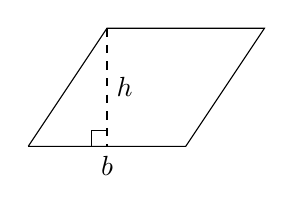
\begin{tikzpicture}
	\draw (0,0) -- node [below,pos=.5]  {$b$} (2,0) -- (3,1.5) -- (1,1.5) -- (0,0);
	\draw [dashed] (1,1.5) -- (1,0) node [pos=.5,right] {$h$};
	\draw (.8,0) -- (.8,.2) -- (1,.2);
      \end{tikzpicture}
    \end{image}
    is
    \[
    A= bh,
    \]
    where $b$ is the length of the base and $h$ is the height of the
    parallelogram. Two vectors $\vec{a}$ and $\vec{b}$ define a
    parallelogram when drawn from the same initial point,
    \begin{image}[2in]
      \begin{tikzpicture}[thick,scale=1.25,>=stealth]
        \draw (.8,0) -- (.8,.2) -- (1,.2);
        \draw (.25,0) arc (0:56:.25);

        \draw [->, ultra thick,penColor2](0,0) -- (2,0);
        \draw [->, ultra thick,dashed,penColor2] (1,1.5) -- (3,1.5);
	\draw (.3,.175) node {\scriptsize $\theta$};
	\draw [->, ultra thick,penColor](0,0) -- (1,1.5);
        \draw [->, ultra thick,penColor,dashed](2,0) -- (3,1.5);
	\draw [dashed] (1,1.5) -- (1,0) node [pos=.5,right] {\scriptsize$h$};
	\node[left,penColor] at (.5,.75) {$\vec a$};
        \node[below,penColor2] at (1,0) {$\vec b$};
      \end{tikzpicture}
    \end{image}
    Trigonometry tells us that $h = |\vec{a}| \sin(\theta)$, hence the
    area of the parallelogram is
    \[
    A = |\vec{a}||\vec{b}|\sin(\theta) = |\vec{a}\cross\vec{b}|,
    \]
  \end{explanation}
\end{theorem}
\begin{question}
  What is the area of the parallelogram spanned by $\vector{1,2,4}$ and $\vector{2,3,1}$?
  \begin{prompt}
  \[
  \text{Area} = \answer{\sqrt{150}}
  \]
  \end{prompt}
  \begin{question}
    What is the area of the triangle spanned by $\vector{1,2,4}$ and $\vector{2,3,1}$?
    \begin{prompt}
    \[
    \text{Area} = \answer{\sqrt{150}/2}
    \]
    \end{prompt}
    \begin{hint}
      This is half of the area of the parallelogram spanned by $\vector{1,2,4}$ and $\vector{2,3,1}$.
    \end{hint}
  \end{question}
\end{question}



\begin{theorem}
  If $\vec{a}$ and $\vec{b}$ are two nonzero vectors, and $\theta$ is
  the angle between them,
  \[
  \vec{a}\cross \vec{b} = \vec{0} \text{ if and only if $\theta=
  0$ or $\theta=\pi$}.
  \]
\end{theorem}

This theorem tells us that the cross product of nonzero parallel
vectors is $\vec{0}$.




\section{Applications}

In addition to the geometric applications we have already seen, we can
also use the cross product in some physical applications.



\subsection{Torque}

Imagine turning a wrench.  The wrench originates at a point $O$ and
terminates at a point $P$.  Let $\vec{r} = \overrightarrow{OP}$.  You
apply a force $\vec{F}$ to the end of the wrench.  If $\vec{F}$ points
in the same direction as $\vec{r}$, the bolt will not twist at all,
since you will just be pulling on the handle.  If $\vec{F}$ is
perpendicular to the handle, then we expect quite a bit of twisting to
occur.

\begin{definition}
  The torque $\vec{t}$ obtained by applying a force $\vec{F}$ to a
  lever arm with position vector $\vec{r}$ is given by
  \[
  \vec{t} = \vec{r} \cross \vec{F} 
  \]
\end{definition}

\begin{question}
  A pipe of length $3 \unit{m}$ has a force of magnitude $2 \unit{N}$
  applied to it as shown below:
  \begin{image}
    \begin{tikzpicture}
      \begin{axis}[
          xmin=-1,xmax=5,ymin=-1,ymax=3,
          clip=false,
          axis lines=center,
          ticks=none,
          unit vector ratio*=1 1 1,
          xlabel=$x$, ylabel=$y$,
          %ytick={-2,-1,...,7},
	  %xtick={-2,-1,...,10},
	  % grid = major,
          every axis y label/.style={at=(current axis.above origin),anchor=south},
          every axis x label/.style={at=(current axis.right of origin),anchor=west},
        ]
        \draw (axis cs:1.13,2.27) arc (63.5:116.5:.3cm);
        \addplot[very thick,penColor,->] plot coordinates {(0,0) (1,2)};
        \addplot[very thick,penColor2,->] plot coordinates {(1,2) (0.5,3)};
        \addplot[very thick,penColor, dashed] plot coordinates {(1,2) (2,4)};
        \node at (axis cs:1, 2.6) [textColor] {\scriptsize$\frac{\pi}{3}$};
        \node at (axis cs:0.6, 0.7) [penColor] {$\vec{r}$};
        \node at (axis cs:0.6, 2.4) [penColor2] {$\vec{F}$};
      \end{axis}
    \end{tikzpicture}
  \end{image}
  Assuming the $z$-axis is coming towards you (out of the page), is
  the torque produced in the positive or negative $z$ direction?
  \begin{prompt}
  \begin{multipleChoice}
    \choice[correct]{positive}
    \choice{negative}
  \end{multipleChoice}  
  \[
  |\vec{t}| = \answer{3\sqrt{3}}
  \]
  \end{prompt}
\end{question}



\subsection{Magnetism} 

When a charged particle moves through a magnetic field, it experiences
a force.  If the charge is $q$, the velocity of the particle is
$\vec{v}$, and the magnetic field is $\vec{B}$, then the force is
given by
\[
\vec{F} = q\vec{v} \cross \vec{B}
\]

\begin{question}
  A particle with negative charge $-2$ enters a constant magnetic
  field given by $\vec{B} = \veci+2\vecj$.  The velocity vector of
  the particle is $\vec{v} = \veck+\veci$.  What is the force
  acting on the particle?
  \begin{prompt}
  \[
  \vec{F} = \answer{4}\veci+\answer{-2}\vecj+\answer{-4}\veck
  \]
  \end{prompt}
\end{question}


\section{The algebra of the cross product}


Below, we summarize some rules for working with cross products:

\begin{theorem}  The following are true for all scalars $s$ and $t$,  and vectors
  $\vec{u}$, $\vec{v}$, and $\vec{w}$ in $\R^3$:
  \begin{description}
  \item[Anticommutativty:] $\vec{v} \cross \vec{w}  = -\vec{w} \cross \vec{v}$.
  \item[Left-distributive:] $\vec{u} \cross (\vec{v} +\vec{w}) = \vec{u} \cross \vec{v}+\vec{u}\cross\vec{w}$.
  \item[Right-distributive:] $(\vec{v}+\vec{w}) \cross \vec{u} = \vec{v} \cross \vec{u}+\vec{w} \cross \vec{u}$.
  \item[Respects scalar multiplication:] $s\vec{v} \cross t\vec{w} = st \vec{v} \cross \vec{w}$.
  \item[Relation to parallel vectors:] $\vec{v} \cross \vec{v} = \vec{0}$
  \item[Orientation:] $\veci \cross \vecj = \veck$, $\vecj \cross \veck = \veci$, and $\veck \cross \veci = \vecj$. 
  \end{description}
  Moreover, these properties determine the cross product uniquely.
\end{theorem}

We will not prove that the cross product is the only function with
these properties, but that is an important point.  If you ever
wondered where this crazy formula came from, this explains it.  If you
want these properties, there is only one operation which does it and
it is the cross product. We leave you with the following curious fact:
The cross product only exists in $\R^3$ and $\R^7$. While this is
beyond the scope of this course, the interested young mathematician can read about it \link[here]{http://www.jstor.org/discover/10.2307/2323537}.







\end{document}
